% !TEX encoding = UTF-8 Unicode
% !TEX program = xelatex

\documentclass[12pt,a4paper,fullpage]{article}
\usepackage{localeng}

\begin{document}

\title{Robust tests: implementation}
\author{}
\date{}
\maketitle


\section{General scheme}

\subsection{Comparing two streams}

All the tests in the suite follow the same scheme. Each of the tests uses some test function that can be applied to a bit stream stream and after reading several bits (the number is determined by the function itself) produces a real number. This procedure is called several times for the file that is tested ($p$ times, producing $p$ numbers) and for the etalon file ($q$ times, producing $q$ numbers). If both data files are generated using truly random bits, then we get a sequence of $p+q$ numbers that are sampled independently from some distribution. This distribution of the numbers depends of the test function chosen and we do not assume anything about it. Instead, using Kolmogorov--Smirnov approach, we sort this sequence of numbers and mark for each of the values where it came from (from $p$ values for the tested file or $q$ values for the etalon file). In this way we get a sequence $S$ that contains $p$ letters <<T>> (test) and $q$ letters <<E>> (etalon), and apply Kolmogorov--Smirnov test for this sequence. Namely, for every prefix of $S$ the numbers $n_T$ and $n_E$ of letters T and E in this prefix are counted, and the deviation $|n_T/p - n_E/q|$ is computed.  We compute the maximal deviation for all prefixes, and then the p-value is returned saying how probable is this --- or bigger --- maximal deviation for a random permutation of $p$ letters~T and $q$ letters~E.

\subsection{Making randomness tests robust}

Used as described, such a test can discover a statistical difference between two sources of bits. If the etalon bits are known to be ``truly random'', then a small p-value indicates that the bits from the tested source do not look random. However, it is still possible that the tested bits are ``truly random'' while the etalon bits are bad, and this situation could also lead to a small p-value provided by the test. 

To avoid this problem, we use the following trick~\cite{shen-robust}: we get $p$ sample values computed using the source that we test, and $q$ values computed using the \texttt{xor} of the etalon bits and (fresh) bits from the test source. In this way we achieve two goals:
\begin{itemize}
\item Whatever the etalon sequence is (assuming it is not correlated with the tested source, e.g., is prepared in advance), the small p-value indicates problems with the tested source. (Indeed,  the \texttt{xor} of a truly random bit with any etalon bit is truly random.)
\item If the etalon sequence is produced by a truly random bit generator, then our test compares the generator we test with truly random bits.
\end{itemize} 
In this way we can adapt randomness tests described in the existing literature making them robust and still preserve most of their ability to detect randomness anomalies. This is what is done in the software (with several known randomness tests; more could and should be added).

\subsection{Technical details}

\begin{description}

\item[Repetitions] After a test is performed as described (and some p-value is produced), we can repeat the procedure if there are enough bits for testing, and get new p-values. Note that (assuming the null hypothesis) this new values are independent, so their product can be used as an aggregated $p$-values.

\item[Dimension]
Some test functions produce not one real value but $d$ real values (for some fixed $d$, called the \emph{dimension} of the test function). Essentially we have here $d$ tests computed in parallel (for example, for efficiency reasons). In this way we get not one p-value, but $d$ p-values computed using the same bits. Note that they are dependent,  and should \emph{not} be multiplied!

\item[Hash values]
Usually the real values produced by test functions do not coincide. Still in some cases this could happen (e.g., if functions have few possible values). To avoid complications when we apply KS-test, we use few more bits taken from the input sequence and produce some has values. The number of hash bits ($32$) is large enough to make the coincidence a red flag by itself.

\item[Approximate KS-values]
The p-values in the Kolmogorov--Smirnov test could be computed using dynamical programming. (There are some approximation formulas, but we avoid them since the approximation errors are hard to estimate and the computation is easy anyway.) Normally the floating-point arithmetic should be precise enough, but if there are doubts, we provide an exact computation with arbitrarily long integers as a backup.
\end{description}

\section{Utility \texttt{rtest}: usage}

The main program (\texttt{rtest.c}, executable file \texttt{rtest}) uses the following options (the equivalent long variants are shown in square brackets after the description):
\begin{itemize}

\item \texttt{-t test\_num} specifies the number of test function used (see the list of all tests and their numbers below) [\texttt{{-}-test}];

\item \texttt{-f test\_file} specifies the name of the file that is tested. The file is understood as a sequence of 32-bit unsigned integers (four consecutive bytes taken from a file form an integer, least significant byte taken first) or a sequence of bytes (the interpretation is determined by a test function used) [\texttt{{-}-file}];

\item \texttt{-e etalon\_file} specifies the name of the file that is used for comparison. If no \texttt{-x} option (see below) is used, then the test function is applied to data from \texttt{test\_file} and \texttt{etalon\_file}; in the robust mode (with \texttt{-x}) the test function is applied to data from \texttt{test\_file} and to the \texttt{xor} of (new) data from \texttt{test\_file} and data from \texttt{etalon\_file} [\texttt{{-}-etalon}];

\item \texttt{-x} requests the robust mode (see above about \texttt{-e} option) [\texttt{{-}-xor}];

\item \texttt{-p num\_samples} specifies the number of times the test function is applied to (fresh) data from tested file (bits from the tested file used for \texttt{xor}-ing are not taken into account) [\texttt{{-}-ptest}];

\item \texttt{-q num\_samples} specifies the number of times the test function is applied to etalon data [\texttt{{-}-petalon}];

\item \texttt{-d dimension} indicates the number of values returned by each call to the test function (different test functions have different dimensions); this number is the number of $p$-values returned by each Kolmogorov--Smirnov two-sample test [\texttt{{-}-dimension}];

\item \texttt{-n number} determines how much data should consumed by each call of the test function; the exact interpretation of this number depends on the test function; some tests ignore this value and decide themselves how many bytes they need; for some other tests only some values of this number are allowed [\texttt{{-}-ntest}];

\item \texttt{-o directory\_name} asks to create files with the list of real values (provided by the test function calls) that were submitted to the Kolmogorov--Smirnov two-sample test, and tells the name of the directory where these files should be created; the directory should not exist before the call. Every Kolmogorov--Smirnov value obtained by the test is accompanied by two files in this directory (that show both samples); one could understand the behavior of the test better when looking at these files [\texttt{{-}-output}];

\item \texttt{-r} requires the test to be repeated; if a positive number is provided as an argument, it is interpreted as the number of repetitions; zero argument means that the test should be repeated as long as there are enough data in the input files [\texttt{{-}-repetitions}];

\item \texttt{-k} requires the exact computation with multi-precision integers for Kol\-mo\-go\-rov--Smir\-nov two-sample $p$-value (instead of long double computation performed by default); can be useful for very large \texttt{-p} or \texttt{-q} options (exceeding $5000$) [\texttt{{-}-ksexact}];

\item \texttt{-v} asks for additional output information (mainly for debugging purposes) [\texttt{{-}-verbose}].
\end{itemize}

There are additional long options (\texttt{sgap}, \texttt{serror}, \texttt{ssize}, \texttt{sdegree}, \texttt{siterations}) that are used by the spectral test (see the description below).

The program runs as long as there are data in the input files or until the required number of repetitions (specified as a non-zero parameter of the \texttt{-r} option) is performed. After one test is performed and several Kolmogorov--Smirnov values are produced and sent to the standard output (the number of these values is the dimension of the test), the testing continues with the rest of the bits in both files.

\section{Tests currently implemented}

Tests are listed according to their test numbers used in \texttt{-t} option; the C name of the corresponding function is shown after the number).

\begin{description}

\item[0] \texttt{all\_bytes}

Dimension $1$, ignores \texttt{-n}, counts the number of bytes that one needs to read to see all $256$ possible bytes (coupon collector problem) if this is not too large (does not exceed some maximal number that is returned otherwise). Uses about 1.5 Kbyte per test value (this number should be multiplied by \texttt{-p} plus \texttt{-q} option parameters for the full test).

\item[1] \texttt{all\_16}

A similar test to the previous one but for $16$-bit integers (pairs of bytes), so it requires much more data ($1.5$--$2$ Mbytes per test value)

\item[3] \texttt{sts\_serial [test\_sts\_serial.c]}

The test depends on two parameters: the number of bits ($n$) analyzed and the maximal length of substrings analyzed ($m$). It produces an array of $3m$ values, i.e., $3$ values for each  integer from $1$ to $m$. For each integer in this range there are two values called $p_1$ and $p_2$ in the NIST document~\cite{nistsp800-22-1a}; we report also one auxiliary ``raw'' value. The value of $n$ is 32 times \texttt{-n} option; the value of $m$ is taken as \texttt{-d} option divided by $3$ (integer part). Requires $n$ bits ($n/8$ bytes, $4$ times \texttt{-n} option), the reasonable application is possible when $n\gg 2^m$ (otherwise the frequencies of factors do not make much sense). 

Let $X$ be the sequence of $n$ bits to be analyzed. For each word $w$ of length at most $m$ we count the number $\textit{count}\,[w]$ of occurrences of $w$ in $X$ (considered as a cyclic word); the sum of all $\textit{count}\,[w]$ for all words $w$ of given length equals $n$. The we compute $\psi^2[k] = (2^{k}/n)\sum_w (\textit{count}\,[w]^2) - n$ where the sum is taken over all strings $w$ of length $k$.
 
For our purposes the values $\psi^2[k]$ (raw values mentioned above) can be used directly, but NIST
 recommends to consider the first and second differences
\begin{align*}
   \Delta\psi[k] &= \psi^2[k] - \psi^2[k-1],\\
   \Delta_2\psi[k] &= \psi^2[k] - 2\psi^2[k-1] + \psi^2[k-2].
\end{align*}   
The \texttt{dieharder} code suggests to let $\psi^2[0]=0$, so $\delta\psi[k]$ is defined for $k\ge1$ and $\delta\psi_2[k]$ is defined for $k\ge2$. (Non-existing values are filled by zeros in the test output).  
 
These numbers are converted to $p$-values according to approximate distributions,
\begin{align*}
    p_1 &= \textit{igamc}\,(2^{k-2},\Delta\psi[k]/2),\\
    p_2 &= \textit{igamc}\,(2^{k-3},\Delta_2\psi[k]/2).
\end{align*}   

\item[4] \texttt{opso [test\_opso.c]}

Original description:~\cite{marsaglia-zaman}. (The \texttt{dieharder} implemenation deviates from the original description in a rather strange ways; we followed the original description). Test consumes $2^{21}+1$ unsigned $32$-bit integers and generates $32-10+1=23$ values according to $23$ possible positions of $10$-bit substrings in a $32$-bit string. For each of $23$ positions we get a word of length $n=2^{21}+1$ in $2^{10}$-letter alphabet. We count $2$-letter words that are \emph{not} factors of this word, and convert this count to a  (presumably uniform) $p$-value assuming normal distribution with some parameters (mean about 141909.33 and $\sigma$ about $290.46$). The \texttt{-n} parameter should be $2097153$ (${}=2^{21}+1$), the \texttt{-d} parameter should be $23$. Uses about $8$ Mbytes per test value.

\item[5] \texttt{oqso [test\_oqso.c]}

The test is similar to \texttt{opso} and is described in the same paper. (Again the \texttt{dieharder} implementation does something rather different.) The difference is that the alphabet contains $2^5$ letters (factors of length $5$ at different positions in the input integers), and we count factors of length $4$ that are missing. Consumes $2^{21}+3$ integers and produces $28$ values. Approximation mean and variance are slightly different ($141909.60$ and $294.656$). The \texttt{-n} parameter should be $2097155$ (${}=2^{21}+3$), the \texttt{-d} parameter should be $28$. Uses about $8$ Mbytes per test value.

\item[6] \texttt{bytedistribs [test\_bytedistribs.c]}

A reimplementation of a test from \texttt{dieharder}, file \texttt{dab\_bytedistribs.c}. From every three $32$-bit numbers from the generator (\texttt{dieharder} allows also generators of different word size, but we assume the size is $32$) one extracts $9$ bytes (three from each integer: $8$ least significant bits, $8$ most significant bits and $8$ bits in the middle). This is repeated $n$ times (specified by \texttt{-n} parameter), so we get $9$ distributions on $\{0,1\}^8$ corresponding to $9$ different byte positions. Then we apply $\chi^2$-square test to the combined distribution on $9\cdot256$ objects with $\textit{ndf}=9\cdot 255$ degrees of freedom (since we have $255$ degrees of freedom for each of $9$ positions). One resulting value is returned (test dimension is $1$). More precisely, each of $256\cdot 9$ counters has expected value $n/256$ and actual value $x$; we compute the sum $S$ of $(x-e)^2/e$ for all counters and then compute the approximate $p$-value as $\textit{gsl\_sf\_gamma\_inc\_Q}\,\,(\textit{ndf}/2, S/2)$. Uses $12$ times \texttt{[-n]} bytes; the \texttt{-n} parameter should be much bigger than $256$ (otherwise the distributions do not make much sense).
     
\item[7] \texttt{knuth\_runs [test\_runs.c]}

Test described in~\cite[p.~65]{knuth2} (the \texttt{dieharder} deviates from it since it considers the first element in a special way, but probably the results do not differ much).  For a sequence of (arbitrary) length $n$ we count the number of parts in its minimal splitting into non-decreasing subsequences (runs). Then we consider $6$-vector consisting of numbers $x_1,\ldots,x_6$ of runs of lengths $1$, $2$, $3$, $4$, $5$, $6$-$\infty$. Then (as explained by Knuth~\cite{knuth2}) one computes
\[
 V=\frac{1}{n}\sum_{1\le i,j\le 6} a_{ij}(x_i-nb_i)(x_j-nb_j),
\]
where coefficients $a_{ij}$ and $b_{i}$ are given by tables provided by Knuth. Test dimension: $2$ (for non-increasing and non-decreasing runs). Uses [\texttt{-n} option] integers ($4\times\texttt{[-n]}$ bytes).

\item[8] \texttt{osums [test\_sums.c]}

This is the ``overlapping sum'' test described in Marsaglia~\cite{marsaglia-diehard} and then included in \texttt{dieharder}~\cite{dieharder} with some changes. Still after some investigation Robert Brown, the author of~\texttt{dieharder}, came to the conclusion that this test should not be used. Still (like any other test function) it provides a correct test if used in a two-samples scheme, so we included it. The test takes any number $m>1$ as size (\texttt{-n} parameter) and uses $2m-1$ input $32$-bit unsigned integers (converted to $[0,1]$ double reals) to produce $m$ overlapping sums (using $m$ integers in each sum). Then some linear transformation (suggested by Marsaglia) is applied to get $m$ presumably independent standard normal variables, they are converted to presumably uniform random variables in $[0,1]$ and Kolmogorov--Smirnov one-sample test is used. The resulting $p$-value is the only test output (dimension is $1$). It seems that for large $m$ there is a significant deviation from the assumed distributions, and Kolmogorov--Smirnov one-sample tests gives small values. So it may be wise to stick to the value $m=100$ as used in original Marsaglia \texttt{diehard} test. Uses about $8\times\texttt{[-n]}$ bytes.

\item[9] \texttt{ent\_8\_16 [test\_ent.c]}

This simple test of dimension $4$ takes arbitrary number $n$ of $32$-bit integer (specified in \texttt{-n} option), and returns four numbers (has dimension $4$). It considers distributions on bytes and $16$-bit integers. For each of these distributions the entropy is computed in a standard way, and also $\chi^2$-test is applied (with $255$ and $65535$ degrees of freedom for $8$ and $16$ bit versions). The four numbers returned are (entropy for $8$ bits, $\chi^2$-test $p$-value for $8$ bits, entropy for $16$ bits, $\chi^2$-test $p$-value for $16$ bits). Note that the values of entropy are less useful for the subsequent analysis since they are usually very close to $8$ and $16$, and measure the deviation from the uniform distribution in a similar way. Uses about $8\times\texttt{[-n]}$ bytes; so \texttt{-n} parameter should be much bigger that $64$ (for bytes) and $32768$ (for $16$-bit integers).

\item[10] \texttt{fftest [test\_fft.c]}

This is a Fourier transform (spectral) test from NIST, as described in~\cite{nistsp800-22-1a}. This description includes corrections from~\cite{kim-umeno-hasegawa}. In this test $n$ integers from the generator are converted into $32n$ bit sequence; this sequence is interpreted as array of $\pm 1$, and discrete Fourier transform is applied. We assume that $n$ is a power of $2$, so the simple algorithm for Fourier transform can be used (taken from \texttt{gsl}, GNU scientific library). In this way we get $n$ complex numbers (since we start with real numbers, only $n/2$ first number are used). We see how many of then have absolute value that exceeds some threshold (namely, $\sqrt{\ln(1/0.05)n}$), the description in NIST document claims that expected value of this number is $0.05n/2$, and the distribution is close to binomial distribution for $n/2$ independent experiments with $0.05$ probability. No derivation for this approximation is given (not to speak about error bounds). It seems that this approximation is quite rough. Figure~\ref{pic:fft-approx} shows the experimental distributions for comparison of some random number generator and its xor with reference generator. One can see that both curves are quite close to each other and quite far from the diagonal (that should appear for uniform distributions). The jumps happen since there are only a few values of the test statistics (the number of values exceeding the thresholds). Let us stress again that the approximation errors do not destroy the validity of test results when using two-sample robust tests.
\begin{figure}[t]
\begin{center}
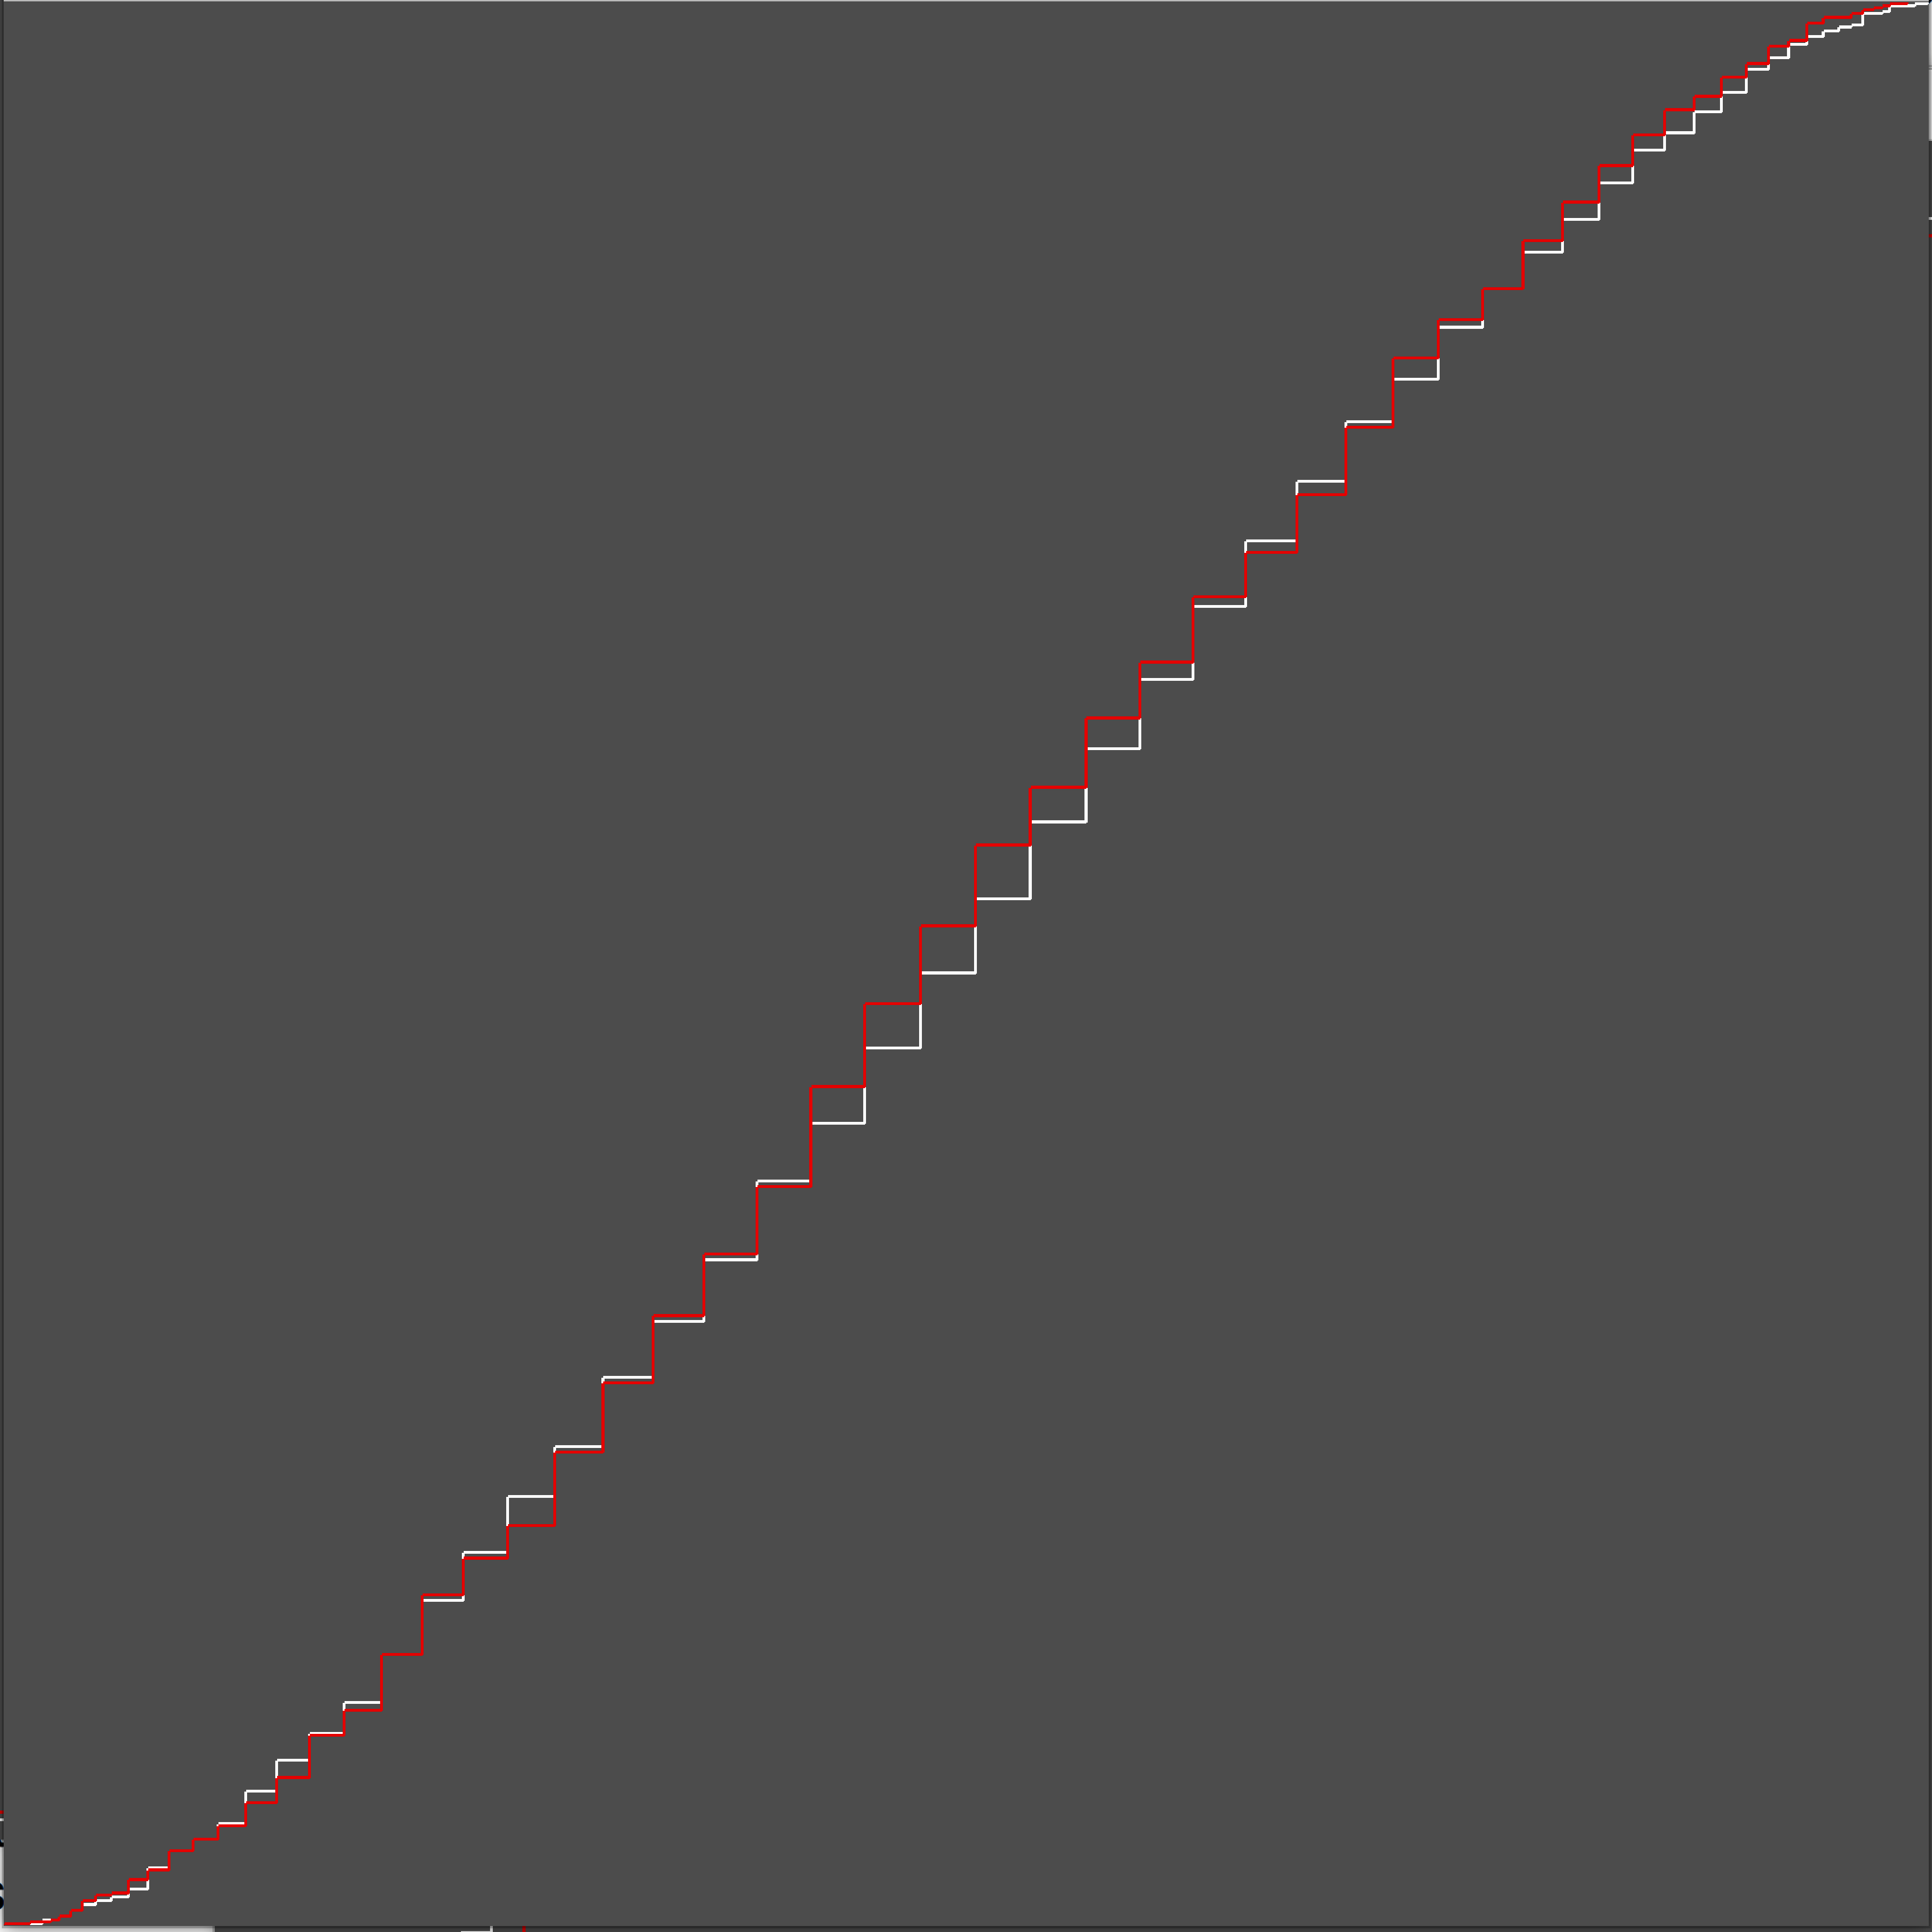
\includegraphics[width=0.4\textwidth]{pdfs/fft-approx.pdf}\qquad
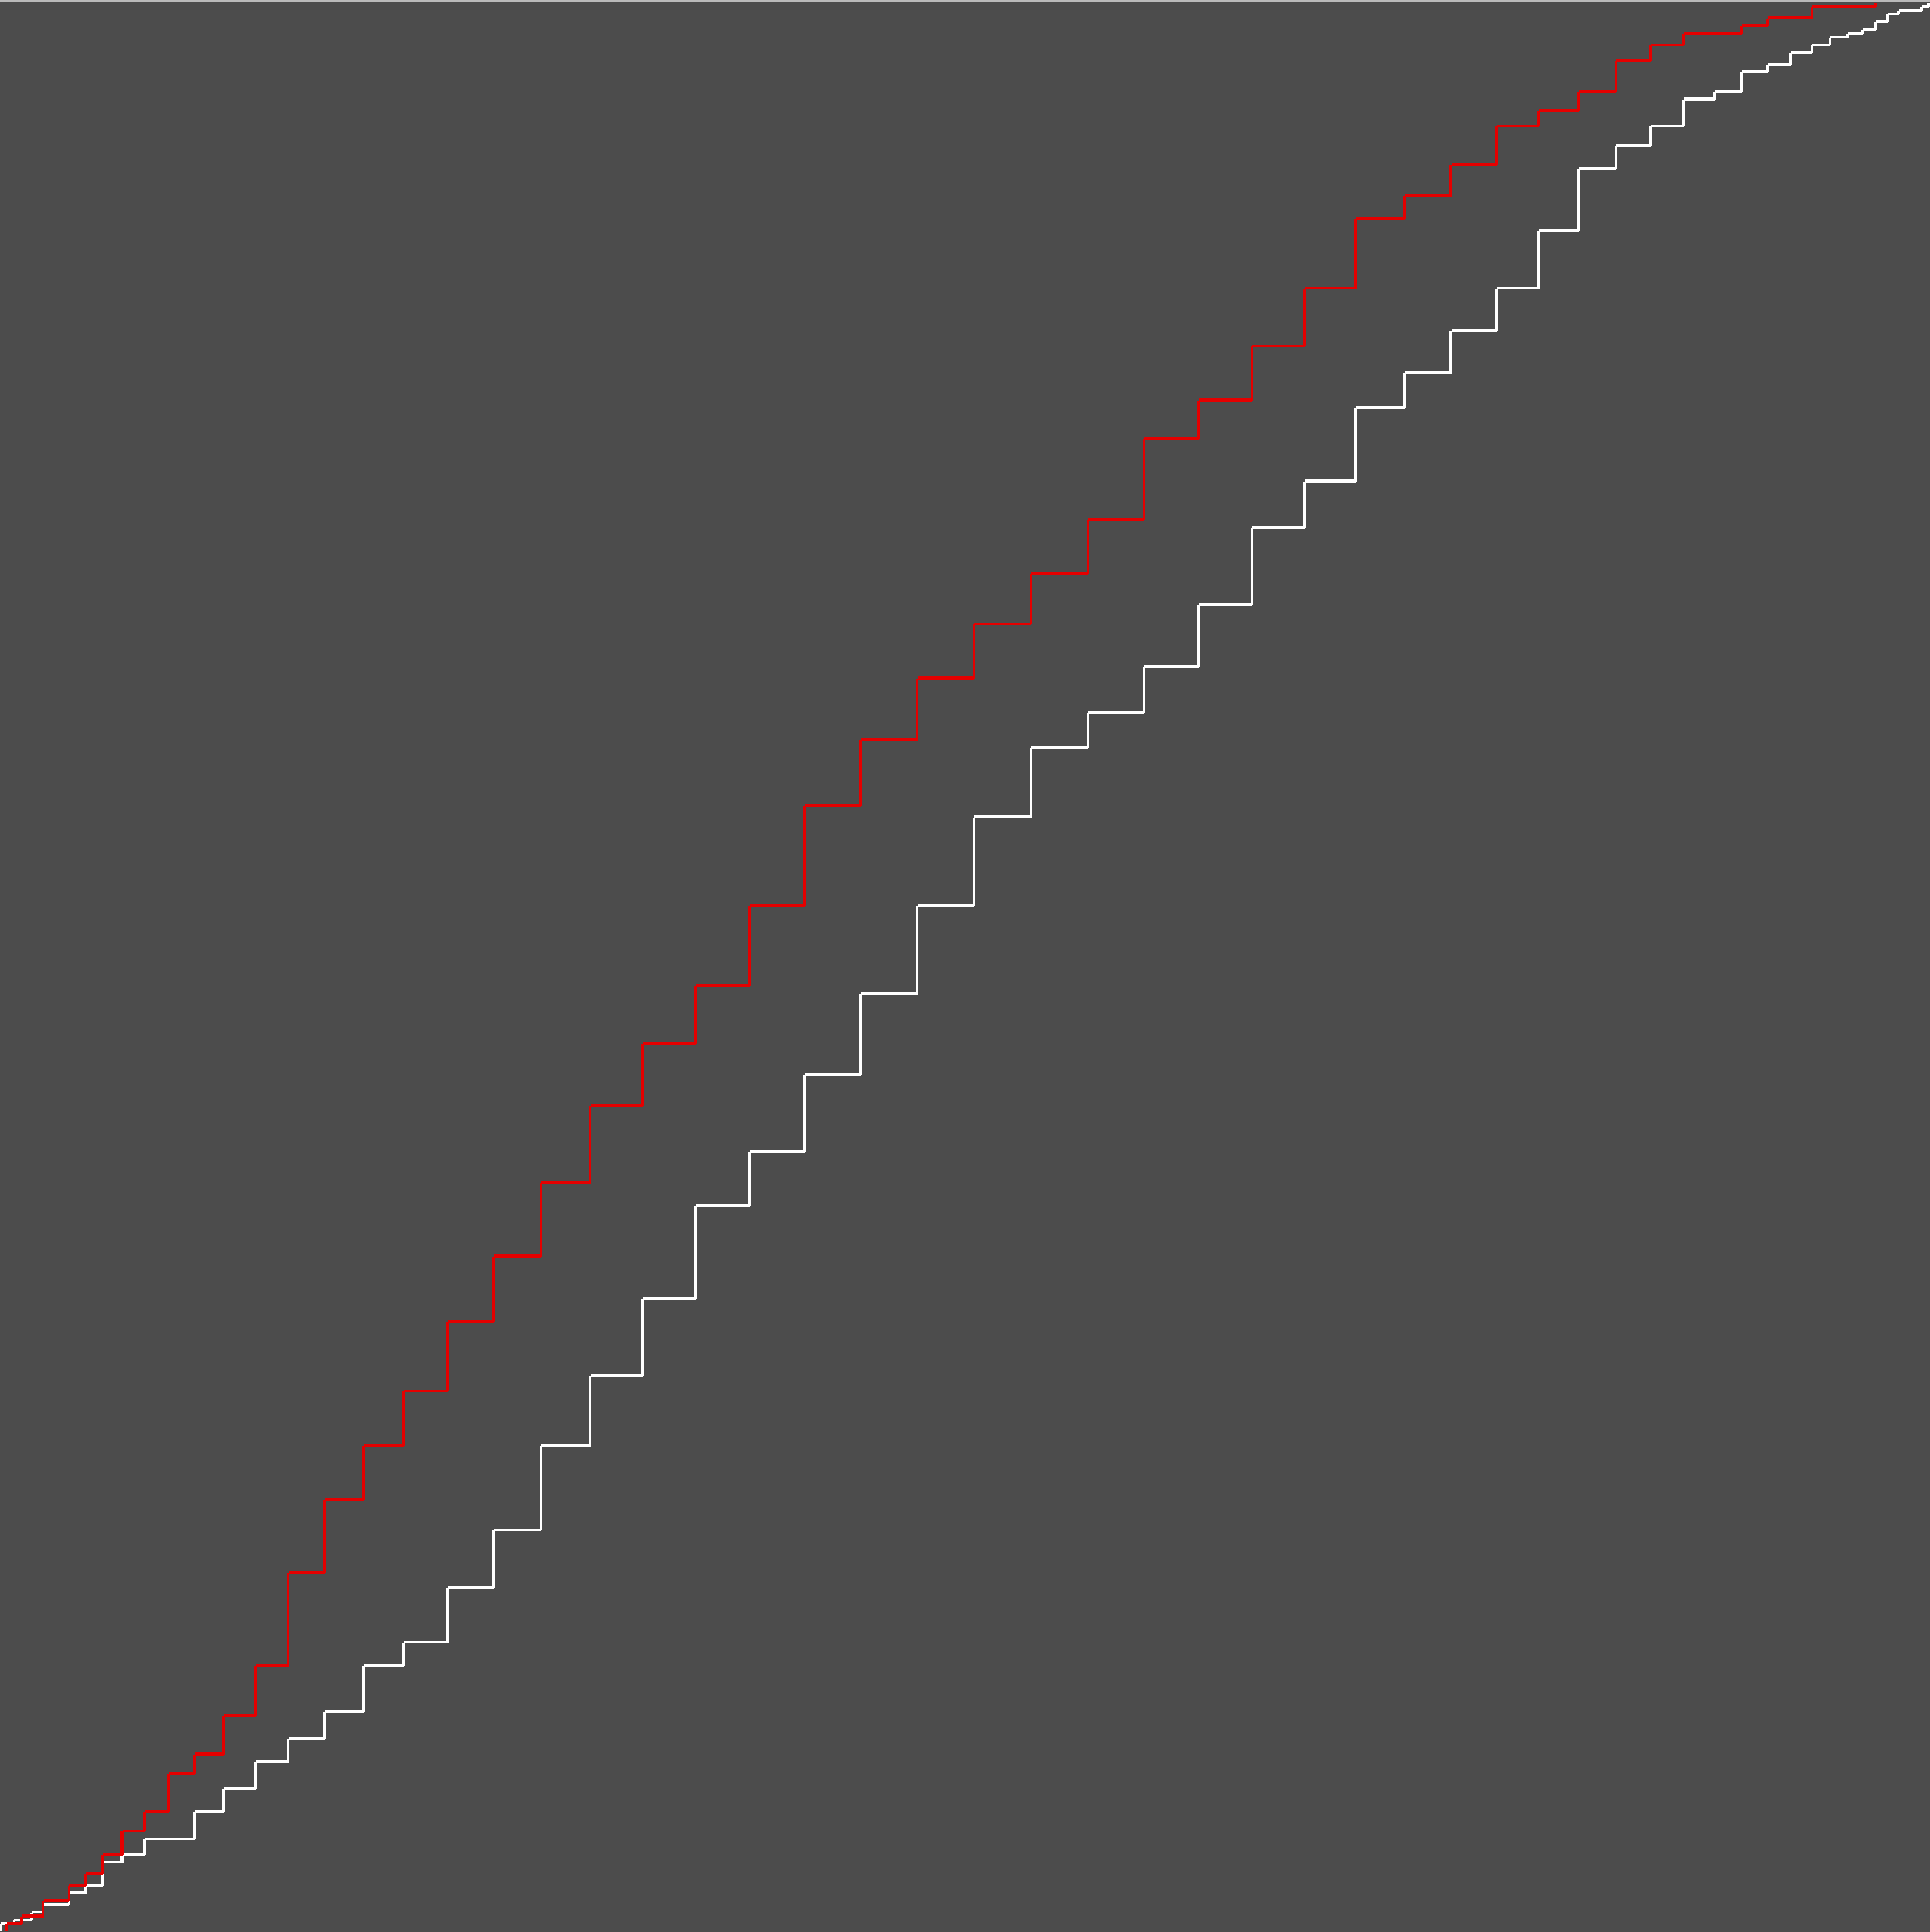
\includegraphics[width=0.4\textwidth]{pdfs/fft-differ.pdf}
\end{center}
\caption{\emph{Left}: the distributions of presumably uniform random variables obtained by Fourier transform test, command \texttt{rtest -x -f a10bis.raw -e ../bitbabbler/raw\_4\_sources -p 1000 -q 1000 -n 256 -t 10 -d 1  -o outfft}. \emph{Right}: a visible difference between test and etalon samples for some bad generator.}
\label{pic:fft-approx}
\end{figure}

Test dimension is $1$, uses $4\times \texttt{[-n]}$ bytes; the \texttt{-n} parameter should be a power of $2$.


\item{11} \texttt{rank32x32 [test\_rank.c]}

This and the following tests (both are implemented in \texttt{test\_rank.c}) check ranks of some matrices . This test has dimension $1$. It forms [\texttt{-n} option] matrices  $32\times 32$ (each uses $32$ integers). Ranks of these matrices are computed and we count the frequencies of ranks $32$, $31$, $30$, [$29$ and smaller]. (This grouping is reasonable since matrices with ranks less than $29$ are rare.) Then the $\chi^2$-statistic is computed and converted to a (presumably) uniform distribution. The same computations are done in  \texttt{dieharder} (while \texttt{diehard} used $31\times 31$ matrices). Uses $128\times\texttt{[-n]}$ bytes.

\item{12} \texttt{rank6x8 [test\_rank.c]}

This test has dimension $25$ (since there are $32-8+1=25$ possible position of a $8$-bit factor in a $32$-bit word). It takes $6\times\texttt{[-n]}$ integers; for each group of $6$ integers it form $25$ matrices $6\times 8$ corresponding to $25$ positions. Ranks are computed, and for each position a distribution of matrices according to ranks ($6$, $5$, [$4$ or less]) is analyzed via $\chi^2$ statistics and transformed into a presumably uniform variable (separately for each position). This follows \texttt{diehard} and \texttt{dieharder} with some corrections, see the discussion in Section~\ref{sec:dieharder-notes}. Uses $24\times\texttt{[-n]}$ bytes.

\item{13} \texttt{bitstream\_o [test\_bitstream.c]}

Both this and the next tests (overlapped and non-overlapped version of a bitstream test from \texttt{diehard} and \texttt{dieharder}) are implemented. This test considers the input stream of bits ($32$ integers are concatenated as written from left to right; the bits are also written from left to right). The test uses $2^{21}+19$ bits (and discard unused bits in the last integer). It consideres all $20$-bit factors in this long string and counts the missing ones, i.e., $20$-bit strings that do not appear as a factor. This number is transformed into a presumably uniformly distributed variable (following \texttt{dieharder}) using empirically observed normal distribution with mean  $141909$ and $\sigma=428$. The dimension of the test in $1$, the \texttt{-n} option parameter should be $2097171$ (number of bits used), or about $256$ Kbytes per test value.

\item{14} \texttt{bitstream\_n [test\_bitstream.c]}

Similar to the preceding test, but non-overlapping $20$-factors are used (the input bit stream is cut into $20$-bit pieces). Uses $2^{21}\cdot 20=41943040$ bits, and this number should be the value of \texttt{-n} parameter; dimension is $1$. Since the words are now independent, the distribution is different, still the \texttt{dieharder} uses the same mean $141909$ with smaller $\sigma=290$.  About $5$ Mbytes per test value.

\item{15} \texttt{lz\_split [test\_lz.c]}

Lempel--Ziv test as it was described in the original version of~\cite{nistsp800-22-1a}. The sequence of bits is split into words according to the following Lemper--Ziv rule: the next word is chosen as \emph{the minimal prefix of the non-processed yet part that is not a prefix of already chosen word}. The algorithm counts the number of full words produced when analyzing $32\times[\text{\texttt{-n} parameter}]$ input bits. The NIST standard suggest some approximation for the resulting distribution in case of $10^6$ bits (\texttt{-n 31250}), so in this case we convert the values to presumably uniform distribution using this approximation. Some problems with this approximation were found in~\cite{kim-umeno-hasegawa}. They can be illustrated by a distribution obtained when applying this test (with NIST parameters) may times to several hardware generators (Figure~\ref{fig:nist-lz}). Still it can be safely used in the two-samples robust version.

\begin{figure}
\begin{center}
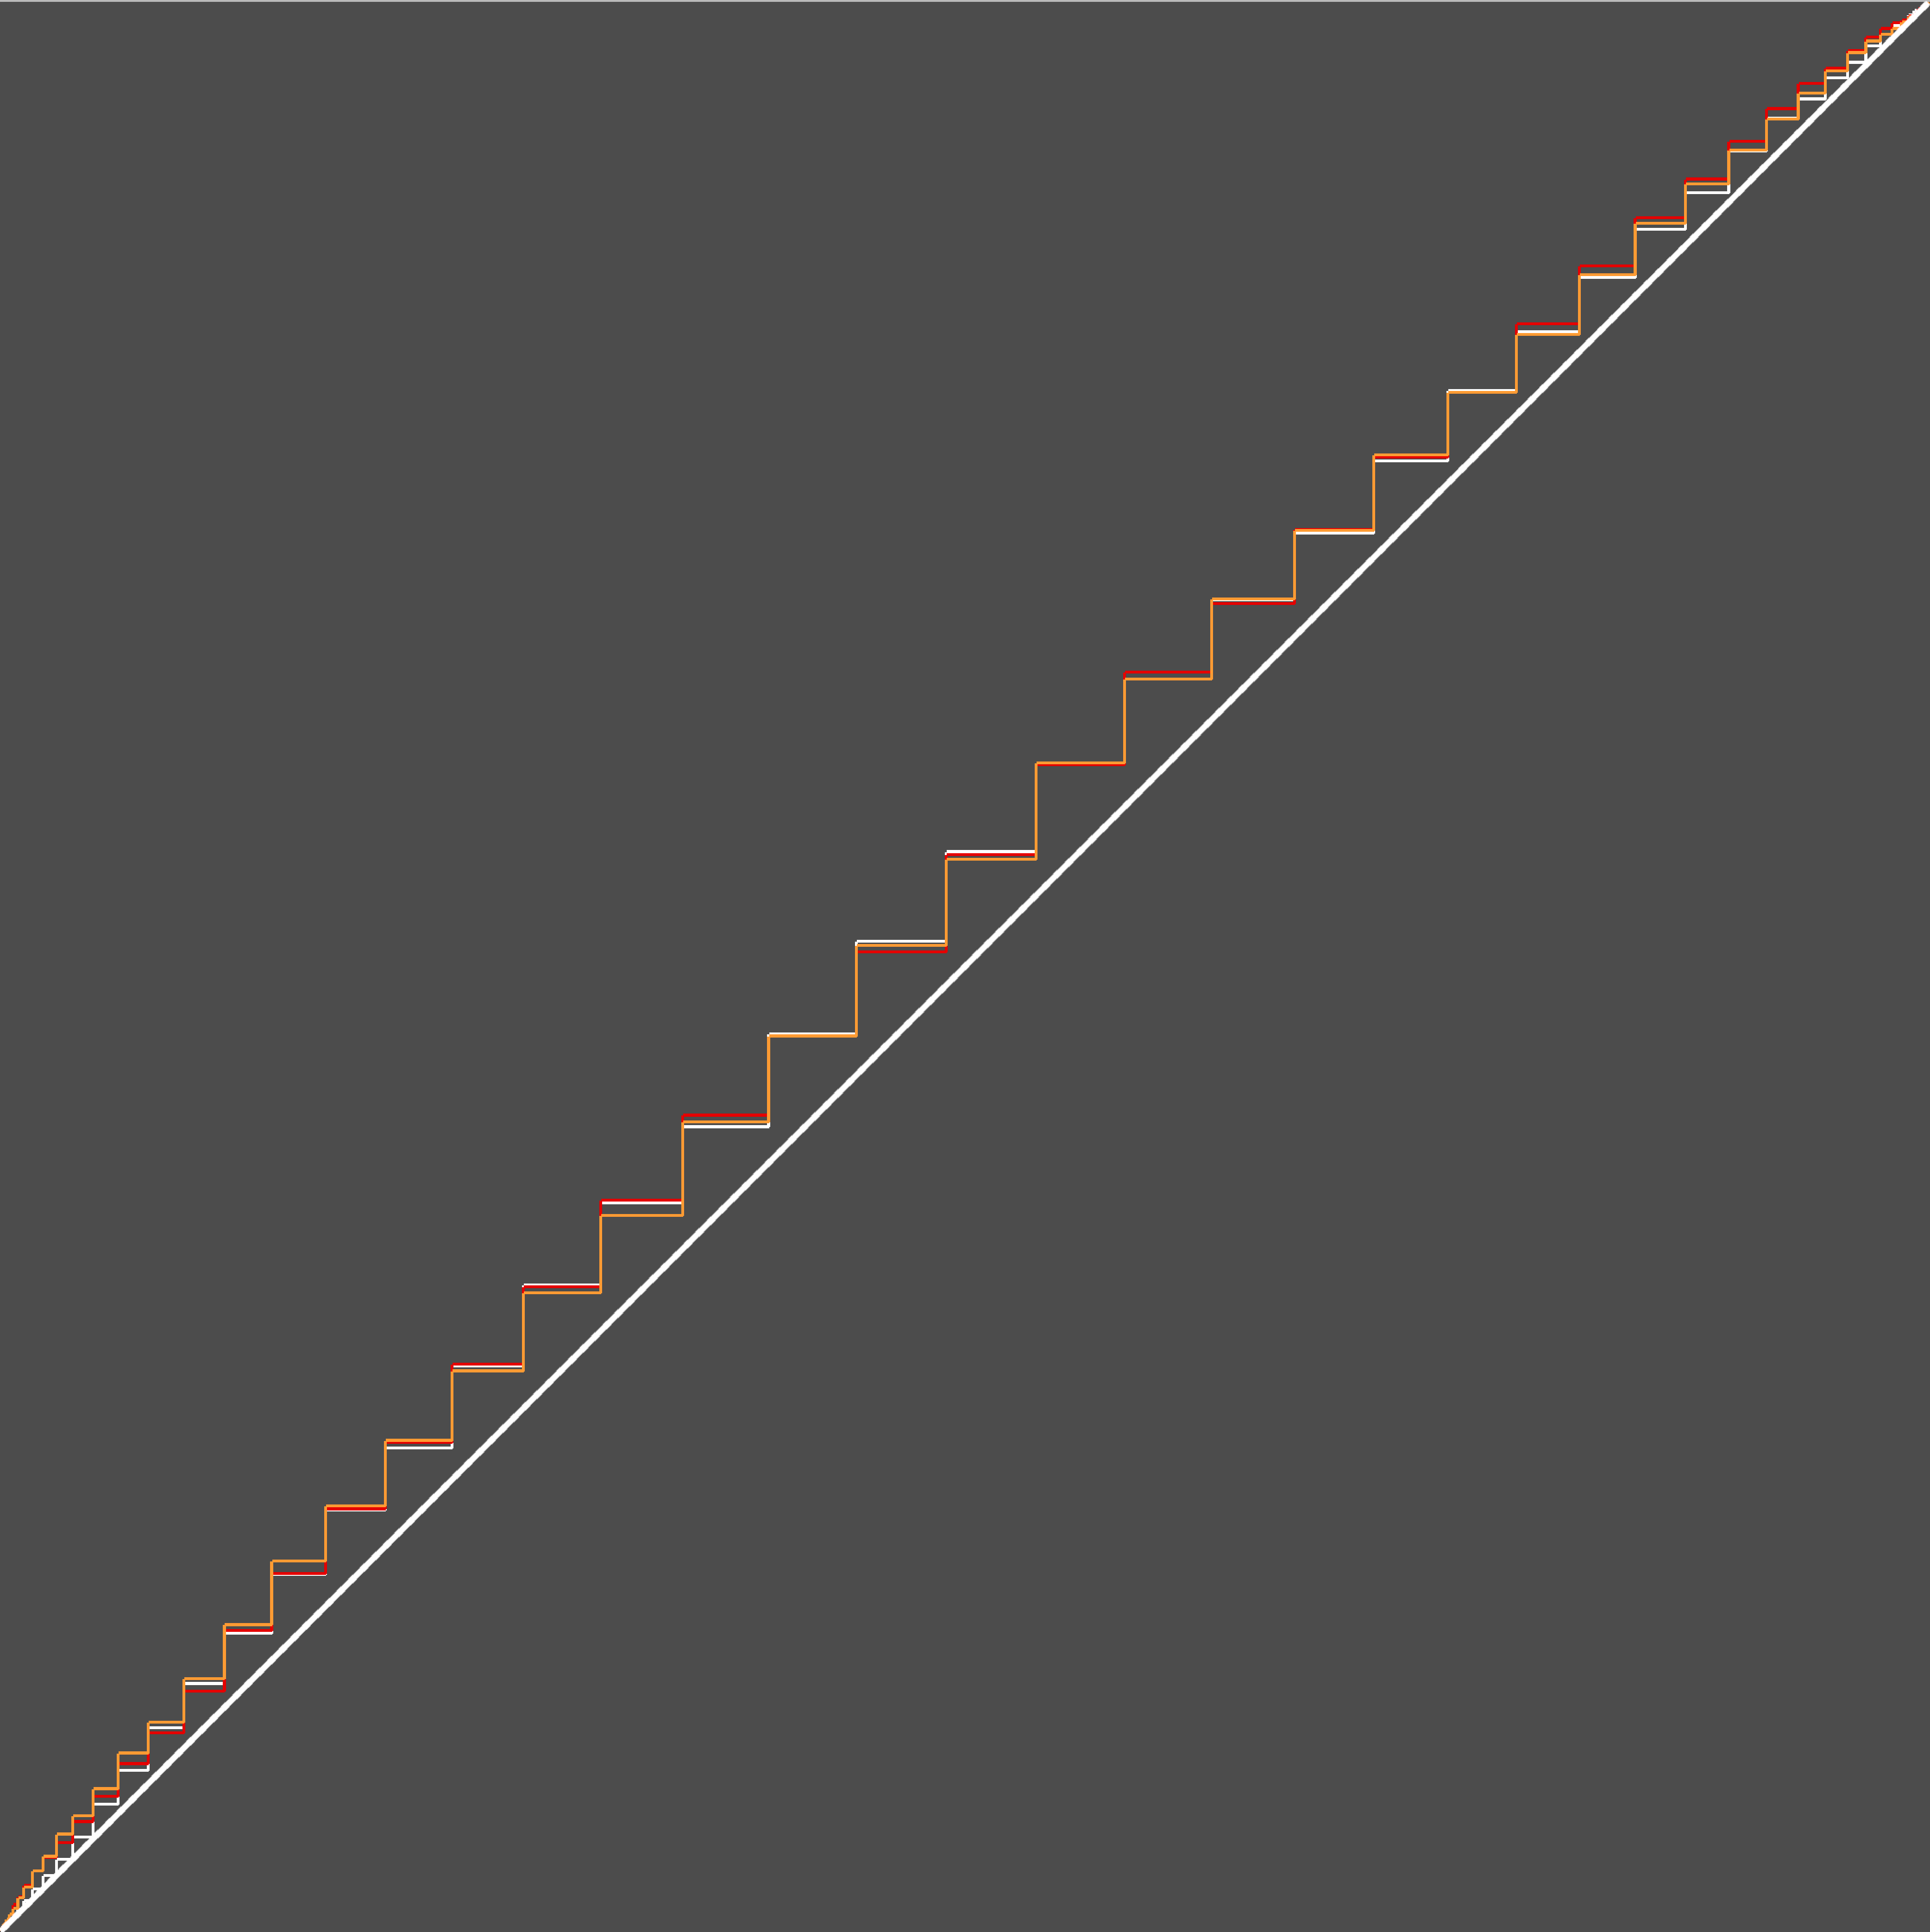
\includegraphics[width=0.6\textwidth]{pdfs/nist-lz.pdf}
\end{center}
\caption{Empirical distributions. Each experiment involved $3000$ Lempel--Ziv decompositions of a bit sequence of length $10^6$; several experiments are shown with different colors. According to the original version of the test, the empirical distribution functions should be close to a diagonal line. One can see both effects mentioned in \cite{kim-umeno-hasegawa}: first, the number of different values is small, and this creates the ``ladder'' structure; second, one can also suspect systematic deviations from the straight line (added for comparison).}
\label{fig:nist-lz}
\end{figure}

\item{16} \texttt{birthdays [test\_birthday.c]}

A ``year'' consists of $2^{24}$ days; we choose $1024$ random days (``birthdays'') and compute $1024$ intervals between birthdays. Some intervals may coincide, and we count the number of coincidences (i.e., the difference between $1024$ and the number of different intervals). We repeat this experiment several times  (\texttt{-n} option) and compare the resulting distribution with presumed approximation (Poisson distribution with $\lambda=16$), getting one $p$-value that is considered as the output of the test. More precisely, we use first $24$ bits from the $32$-bit integers from the input sequence; this gives us one $p$-value, than next $24$ bits from the same $32$-bit integers, and so on ($32$ cyclic shifts, as described --- but not implemented --- in \texttt{dieharder}). The test dimension is $32$, and it uses $1024$ times [\texttt{-n} option] integers ($4096\times \texttt{[-n]}$ bytes) for each set of $32$ values. Note that the test is robust (as any other two-sample test) but its usefulness is not clear (due to the systematic deviation of the observed distribution from the presumed one, see Section~\ref{sec:dieharder-notes}, Figure~\ref{pic:birthdays}).

\item{17} \texttt{mindist2d [text\_dist2d.c, minimal\_distance.hpp]}

This test has dimension $2$. First, it uses $2n$ (where $n$ is \texttt{-n} parameter) unsigned $32$ bit integers (scaled to $[0,1]$) to construct $n$ points in the unit square. Then it computes the distance between two closes points. The same is done for $2n$ points obtained as follow: each $32$-bit integer is cut into two halves, and two resulting unsigned $16$-bit integers determine a point in the unit square. The algorithm uses $O(n\log n)$ algorithm of divide and conquer type for finding the minimal distance (the debug output includes also the computations with exchanged coordinates and a naive algorithm result; all three should be the same).

Originally, the minimum distance test in \texttt{diehard} used $8000$ random points in the square of side $10000$, and used some approximation to transform the minimal distance into an (approximately) uniform distribution; then a one-sample Kolmogorov--Smirnov test was applied to $100$ values of this distribution. The \texttt{dieharder} suite uses an improved approximation (that we do not need because of using robust two-sample testing).

\item{18} \texttt{spectral}

This test has several parameters provided as long options. The parameter \texttt{{-}-ssize} is the number of vertices in a random undirected graph constructed by this test. The parameter \texttt{{-}-sdegree} is the average degree of the graph. It should be an even number $d$; then for each vertex we add $d/2$ random edges incident to this vertex (the other endpoints are uniformly distributed; multiple edges and loops are allowed). Then we apply the procedure that estimates the second eigenvalue for a random walk on a graph, written by Yan Ollivier~\cite{ollivier}. This is an iterative algorithm that has some parameters. It constructs lower and upper bounds for the second eigenvalue and stops when the difference between them becomes smaller than the \texttt{{-}-sgap} parameter. The algorithm is probabilistic and makes an error (provides invalid bounds) with probability at most \texttt{{-}-serror} parameter. However, we use some simple fixed pseudo-random sequence instead of the random bits, since our \texttt{xor}-trick guaranteed correctness of $p$-values independently of the function used for testing. Another parameter (an integer) is the maximal number of iteration allowed for Ollivier's algorithm; it is provided by the long option \texttt{{-}-siterations}. 

Note that this test is valid for any values of this additional parameters: the bounds for the eigenvalues (even if they are not actually bounds) can be used as well as true eigenvalues.  There were some cases in our experiments when taking the smaller error and gap parameters made the test \emph{less} sensitive (and longer) --- though in other cases smaller error and gap made the test more sensitive.

There is also a standalone version of these tests (described shortly in the next section).

\end{description}

For convenienve we also provide  some shell scripts that run these tests for suitable parameters (adjusted for $1$~Mb, $10$~Mb, $100$~Mb, $1$~Gb, $10$~Gb files). Some tests take a long time, so it may have sense to delete some tests from these files if they take too much time. Two arguments are required: the name of the tested file and the name of the reference file.

A short reminder to be taken into account when interpreting the test values:

\begin{itemize}

\item The $p$-values produced by these files are reliable (not based on any unproven assumptions about the tests and/or approximations\footnote{The only compromise here happens when we use floating point numbers for computing the Kolmogorov--Smirnov value; looking at the output of \texttt{ks2compare} utility, we may hope that this does not create any problems for samples of size up to $5000$, but one should be careful before pronouncing the final verdict and use option \texttt{-k} that asks for an exact computation.}). For any given test this means that for every $p>0$ and for every reference file the probability of the event ``the test with random bits in the tested file will produce value at most $p$'' is at most $p$. Note also that the tests never ``rewind'' the file (using the same bits several times): if there is not enough bits in the file, no value is produced.

\item There is no claim of uniform distributions for the test output (for a random bits input), so \emph{output values close to $1$ do not indicate any problems}.

\item The tests (some individual tests and the shell scripts) produce many numbers at once. These number are not independent. So one should \emph{not} multiply them to get a more impressive number. Moreover, one should apply the Bonferroni correction (that makes the conclusion less impressive): If for a chosen family of tests \emph{one} of $m$ number (where $m$ is the total number of outputs, depending on the chosen family) is $p$, the resulting $p$-value is $mp$.  For example, if one of the $40$ test values is less than $0.01$, one should not become suspicious about the generator, since $40\cdot 0.01$ is $0.4$, definitely not enough to start worrying.

\item On the other hand, if you repeat some test several times (say, using \texttt{-r} option, or just applying it to different runs of the same random bit generator), the output values \emph{are} independent. This can be used to amplify the non-randomness conclusions. For example, if a test (or a group of tests) fixed before the experiment produces $37$ values, we made $15$ runs with the same generator (and the same or different reference files, fixed in advance), and it turned out that one of $37$ values is less than $0.001$ for all the experiments, the correctly computed $p$-values is $37\cdot(0.001)^{15}$. One should distinguish this from the other case: for each of $15$ experiments there is some output value less than $0.001$, but this value can be produced by different tests in different experiments. In this case the correct computation of $p$-value gives $(37\cdot0.001)^{15}$.

\item The recommended approach when discrediting some generator: make some preliminary experiments to determine which tests look more suspicious. Then try the selected test on the fresh input from the generator and report the $p$-value obtained for this test. But be careful if a small $p$-value appears after several attempts to discredit the generator: a honest researcher should multiply the resulting $p$-value by the number of attempts.

\end{itemize}

\section{Spectral tests}

This section describes a standalone version of spectral tests that can be useful for someone who wants to modify the program and do not worry about the general structure of robust tests.

The spectral tests currently involve a lot of parameters, so they are not yet included in the robust testing suite. Currently we do \emph{not} have examples where they beat all the other tests in the sense that they find some deficiency in a generator that cannot be found by other tests. Still it would be desirable to have more robust tests especially if they use different approaches.

The call
\begin{verbatim}
example -g gap -e err -s size -d deg -o iter -n number -l -u -h] filename
\end{verbatim}

The utility \texttt{example} analyses one file with name \texttt{filename} (so this utility should be combined with the \texttt{xoring} made separately to get a robust test). It uses bytes from this file to construct a sequence of graphs. The size of the graph is determined by option parameter \texttt{-s size}; it should be a power of $2$ not exceeding $65536$. Each (undirected) graph is constructed by emitting \texttt{deg} random edges from each vertex. (Note that the resulting undirected graph may not have constant degree, but the average degree is close to $2\cdot\texttt{deg}$.) Then the algorithm from~\cite{ollivier} is used to compute the second eigenvalue for the resulting graph. This is an iterative algorithm that has some parameters. It constructs some lower and upper bounds for the second eigenvalue and stops when the difference between them becomes smaller than \texttt{gap} (\texttt{-g} parameter). Also it uses some internal randomness (now crudely replaced by some fixed pseudo-random generator\footnote{Since our \texttt{xor}-trick guaranteed correctness of $p$-values independently of the function used for testing, we decided to use some simple pseudo-random sequence with fixed seed.}. Also the algorithm uses some upper bound for the number of iterations that can be specified by option \texttt{-o}. The option \texttt{-n} parameter specifies the maximal number of graphs that should be constructed (if there is enough bits in the input file \texttt{filename}).

The output of the utility is a sequence of lines. Each of them corresponds to one graph, and the contents of the lines is determined by the options \texttt{-l,-u,-h} (at least one of them should be present). The output line contains
\begin{itemize}
\item the lower bound for the second eigenvalue, if \texttt{-l} is present;
\item the upper bound for the second eigenvalue, if \texttt{-l} is present;
\item some hash value (useful for tie breaking), if \texttt{-h} is present.
\end{itemize}
Also an option \texttt{-v} (verbose) can be used to provide more information.

\section{Other tools}\label{sec:graphic}

There are few simple tools that visualize data from \texttt{.wav} and raw data files and perform conversion between formats.

\begin{itemize}
\item \texttt{readwav [-m|-s|-y] filename.wav} shows data (signal readings interpreted as signed integers) from a \texttt{.wav} file. For a stereo file \texttt{[-s]} it takes values from both channels and draws a pair. The option \texttt{[-y]} does the same but corrects the $1$-sample lag in the right channel (that happens in Yamaha~MW10 and Behringer~1204USB mixers we used); mono signal has identical readings in both channels after the correction. The \texttt{[-m]} option splits the movo \texttt{.wav} file into pairs of sample values (signed integers) and draws the corresponding points. The number of bits per value should be $8$, $16$ or $24$.

\item \texttt{getdatawav [-m|-s|-y] source.wav dest1 [dest2]} converts standard \texttt{.wav} file into raw format, deleting the header and splitting stereo data into two separate files. Options \texttt{-s} and \texttt{-y} require two destination files (\texttt{dest1} is for the left channel, \texttt{dest2} is for the right channel). Option \texttt{-m} is used for mono files, and just deletes the header. The input file should have resolution $8$, $16$, or $24$. The order of bytes remains unchanged.

\item \texttt{drawpair -b num\_bytes -l|-m -c} draws pairs obtained from two files (in parallel) or from one file (\texttt{-c}; two consecutive data form a pair). The \texttt{num\_bytes} parameter gives the number of bytes interpreted as a signed integer; \texttt{-l}/\texttt{-m} option (one of two should be present) says whether the integers are assumed to appear in \texttt{l}east or \texttt{m}ost significant byte first.

\end{itemize}

\section{Two-source extractor tools}\label{sec:2-extractor}

We implemented the two-source extractor described in Section~\ref{sec:two-sources}. We used the finite field of size $2^{1024}$ whose elements are represented as polynomials in $\mathbb{F}_2[x]$ considered modulo
\[
p(x)=x^{1024}+x^{19}+x^{6}+x+1.
\]
This polynomial is suggested as low-weight irreducible polynomial in~\cite{fields}. ``Low weight'' means that only a few coefficients are non-zero; this allows us to simplify the division modulo this polynomial.  We used the natural basis 
\[
1, x, x^2,\ldots, x^{1023}
\]
in the field (the quotient of $\mathbb{F}_2[x]$ modulo $p(x)$); the multiplication by the basis elements can be obtained by repeated multiplications by $x$. And a multiplication by $x$ is just a shift in the array of coefficients, followed by a reduction modulo $p(x)$. This reduction is applied to a polynomial of degree $1024$; we have to change coefficients in the degrees involved ($20$, $7$, $2$, $1$). This simple operations are implemented in file \texttt{extract.c}; we produce a bit string of length $128$ from two strings of length $1024$ (the field elements).

The file \texttt{extractor.c} calls this extraction function. Since in our experiments we used \texttt{.wav} files where most significant bits (of a $16$-bit words from analog-digital converter are often zeros), we decided to use \texttt{xor} of two halves of an $16$-bit word to get $8$ bits that have (hopefully) reasonably high min-entropy. The command 
\begin{verbatim}
extractor file1 file 2
\end{verbatim} 
applies this operation (\texttt{xor}ing of two bytes in a $16$-bit integer) to each of files \texttt{file1}, \texttt{file2}, applies the extractor function as described, and send the resulting bits to standard output. 

In this way from $2048+2048$ bits from both files we generate $1024+1024$ bits (by \texttt{xor}ing), and then generate $128$ output bits, so the production rate is $1:32$ (one output bit for $32$ input bits).

\begin{thebibliography}{9}

\bibitem{dieharder}
Robert G.~Brown, \emph{\textup{Die}Harder: \textup{A Gnu Public License Random Number Generator}}, version 3.31.1.  \url{http://www.phy.duke.edu/~rgb/General/dieharder.php} (2006--2018).

\bibitem{kim-umeno-hasegawa} 
Song-Yu Kim, Ken Umeno, Akio Hasegava, \emph{Corrections of the NIST Statistical Test Suite for Randomness}, \url{https://eprint.iacr.org/2004/018.pdf}.

\bibitem{knuth2}
Donald Knuth, \emph{The Art of Computer Programming. Volume 2. Seminumerical Algorithms}. Second edition, Reading et al., Addison--Wesley, 1981. ISBN 0-201-03822-6.

\bibitem{marsaglia1985}
George Marsaglia, A Current View of Random Number Generators, \emph{Computer Science and Statistics, Sixteenth Symposium on the Interface}, Elsevier, North-Holland (1985), 3--10.

\bibitem{marsaglia-diehard} 
George Marsaglia, \emph{Random Numbers CDROM including the Diehard Battery of Tests of Randomness}, 1995, was available at \url{http://stat.fsu.edu/pub/diehard/}; now (2019) still avaliable as snapshots from \url{https://web.archive.org}. Contains the preprint version of~\cite{marsaglia-zaman,marsaglia1985}

\bibitem{marsaglia-tsang}
George Marsaglia, Wai Wan Tsang, Some difficult-to-pass tests of randomness, 
\emph{Journal of Statistical Software}, \textbf{7}(3), 2002, \url{https://www.jstatsoft.org/article/view/v007i03}.

\bibitem{marsaglia-zaman}
George Marsaglia, Arif Zaman,  Monkey Tests for Random Number Generators, \emph{Computers and Mathematics with Applications}, \textbf{26}(9), 1--10 (November 1993).

\bibitem{nistsp800-22-1a} % 
NIST Special Publication 800-22:  Andrew Rukhin, Juan Soto, James Nechvatal, Miles Smid, Elaine Barker, Stefan Leigh, Mark Levenson, Mark Vangel, David Banks, Alan Heckert, James Dray, San Vo, \emph{A Statistical Test Suite for Random and Pseudorandom Number Generators for Cryptographic Applications}, Revised: April 2010, Lawrence E.~Bassham III,
National Institute of Standards and Technology, Technology Administration, U.S.~Department of Commerce (NIST),  Revision 1a (2010), 131 pp., {\scriptsize\url{https://www.nist.gov/publications/statistical-test-suite-random-and-pseudorandom-number-generators-cryptographic}}. Previous version seems to be unavailable at this site, but the review of Elaine B. Barker, \emph{ITL Bulletin, December 2000, 3~pp.} is available at \url{https://tsapps.nist.gov/publication/get_pdf.cfm?pub_id=151231}. The Lempel--Ziv test, criticised in~\cite{kim-umeno-hasegawa}, was there (\#10) according to the review; it is missing in the updated version.

\bibitem{ollivier}
Yann Ollivier,  \emph{Spectral gap of a graph}, a public domain code for finding the spectral gap of a graph,  \url{http://www.yann-ollivier.org/specgraph/specgraph} (2004)

\bibitem{shen-robust}
Alexander Shen, \emph{Making randomness tests more robust}, HAL archive, 2018, \url{https://hal.archives-ouvertes.fr/hal-01707610}.


\end{thebibliography}



\end{document}
Implementation remarks: the main driver file is \texttt{rtest.c}; the definitions for the test functions are given in \texttt{test\_func.c} and additional files (see the macro \texttt{TESTS\_C} in the \texttt{Makefile}). To add a new test function, one should put its code in a \texttt{.c} file, put its forward definition in \texttt{test\_func.h} and add it to the list of all test functions in \texttt{test\_func.c}. Some tests use \texttt{c++} code (see the \texttt{Makefile}). 

We used hashes in a different way to simplify the code structure: the function returns not only some values (the number of returned values is the dimension), but also returns $64$ bits (two $32-bit$ integers) that are used to resolve the ties: if the test function returns two identical values, these hash values are compared for sorting. Normally $64$ bits should be enough to resolve the ties (if this does not happen, this means that the file we are testing is not random enough, so it creates a failure by itself).

The tools to compute the Kolmogorov--Smirnov $p$-values (for two samples; some tests also use calls to Kolmogorov--Smirnov distribution function for one sample) are taken from another directory (see \texttt{KS\_C} macro definition in \texttt{Makefile}).

